\documentclass[11pt]{article}
\usepackage[review]{acl}

\usepackage{times}
\usepackage{latexsym}
\usepackage[T1]{fontenc}
\usepackage[utf8]{inputenc}
\usepackage{microtype}
\usepackage{inconsolata}
\usepackage{graphicx}
\usepackage{amsmath}
\usepackage{amssymb}
\usepackage{booktabs}
\usepackage{multirow}
\usepackage{placeins}
\usepackage{tikz}
\usepackage{pgfplots}
\pgfplotsset{compat=1.18}
\usepgfplotslibrary{groupplots}
\usetikzlibrary{arrows.meta,calc,positioning}

\newcommand{\system}{ProactMem}
\title{Proactive Memory for Event-Driven LLM Agents}
% Review mode suppresses author identities. The AAMAS source retains the
% author list for a future accepted, non-anonymous version.
\author{Anonymous ACL submission}

\begin{document}
\maketitle

\begin{abstract}
Proactive LLM agents anticipate service opportunities from ongoing observations and accumulated history.
A central challenge is determining which historical observations remain applicable to the current event and can support a timely service decision.
We propose Proactive Memory (\system{}), combining bounded recent events, source-checked temporal trajectories, and replay-assessed behavioral regularities.
The trajectory validation step checks extracted facts against source events, while historical replay assesses recurring regularities before they are matched to current events.
We also construct ProactiveStream, a longitudinal benchmark covering three application scopes, where agents process isolated event streams chronologically under episode-aware opportunity labels.
\system{} achieves higher effectiveness than the evaluated external baselines in every scope.
Ablation studies support the contributions of hierarchical memory organization and validation to service-opportunity detection.
\end{abstract}

\section{Introduction}
\label{sec:introduction}

LLM agents are extending task execution toward proactive assistance that identifies service opportunities from ongoing observations and accumulated history.
In activity support, smart homes, and software collaboration, useful assistance depends on recognizing new needs, selecting relevant historical evidence, and tracking prior assistance.

Existing work develops proactive decisions and agent memory.
ProactiveAgent learns task proposals from activity contexts~\citep{lu2025proactiveagent}; ContextAgent combines sensed context with historical personas~\citep{yang2025contextagent}.
Mem0 consolidates and retrieves information~\citep{chhikara2025mem0}, while A-MEM links historical notes~\citep{xu2025amem}.
ProactiveBench and ContextAgentBench evaluate task proposals and contextual service; LoCoMo and LongMemEval assess long-term conversational memory~\citep{maharana2024locomo,wu2025longmemeval}.
Continuous assistance also requires assessing memory accumulation, current applicability, and changing opportunities within one event stream.
This raises a central question: \emph{how can history become source-grounded, historically supported, and currently applicable memory for timely, selective assistance?}

To study this question, we construct \emph{ProactiveStream}, a longitudinal event-stream benchmark spanning Sports, Home, and Code.
Agents build memory chronologically within isolated participant, home, and repository streams, assessing each opportunity's first actionable window and subsequent changes.
With a shared backbone and intervention control policy, existing methods show different trade-offs between opportunity recovery and false interventions (Table~\ref{tab:main_results}).
Figure~\ref{fig:intro_scenario} links earlier evening walks to current assistance.

\begin{figure}[!b]
    \centering
    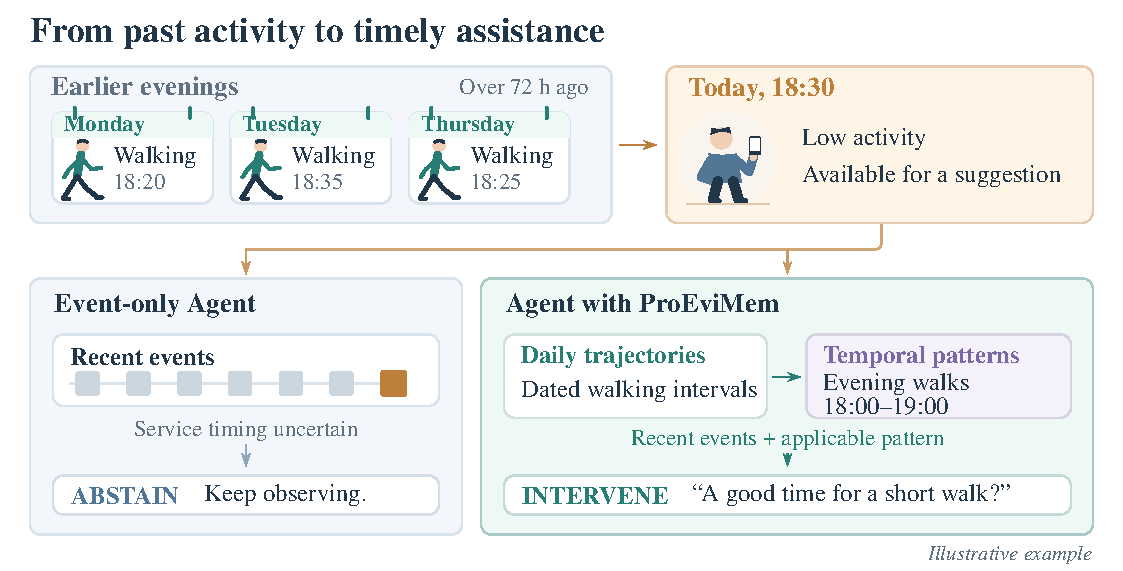
\includegraphics[width=0.96\columnwidth]{Fig_Intro_Scenario.pdf}
    \caption{Illustrative Sports scenario. \system{} retrieves a supported evening-walk regularity to guide assistance beyond recent events.}
    \label{fig:intro_scenario}
\end{figure}

We propose Proactive Memory (\system{}; Figure~\ref{fig:architecture}), linking recent observations, temporal activities, and recurring behavior.
Event memory preserves recent evidence; temporal trajectory memory abstracts source-grounded activities; behavioral regularity memory captures supported conditional behavior.
Together, these layers connect immediate changes with long-term context.

LLMs construct cited trajectories from completed events, followed by source validation of typed facts.
Historical replay assesses regularities inferred from these trajectories.
At decision time, semantic screening uses memory relevance and event-local abstention evidence to route the event.
Full assessment combines recent events, trajectories, and applicable regularities to judge service value.
Intervention control filters repeated proposals; the finalized decision precedes event commitment and memory updates.

Our contributions are:
\begin{itemize}[leftmargin=*, itemsep=0pt]
    \item ProactiveStream supports longitudinal evaluation of memory formation and repeated service decisions, preserving causal history, entity isolation, and episode-aware reference opportunities across three scopes.
    \item \system{} combines source-checked trajectory abstraction, replay-based regularity assessment, and selection of currently applicable regularities to supply historical context for proactive service decisions.
    \item \system{} uses long-term behavioral context to identify service opportunities missed by recent events alone and support more selective intervention decisions.
\end{itemize}

\section{Problem Formulation}
\label{sec:problem}

\subsection{Events, Habits, and Decisions}

Let a session be an ordered stream of events $E=(e_1,\ldots,e_T)$.
Each event is represented as
\begin{equation}
e_t=(\tau_t,a_t,v_t,o_t,m_t)
\end{equation}
Here, $\tau_t$ is time, $a_t$ is the actor, $v_t$ is an action verb, $o_t$ is an object or entity, and $m_t$ contains domain metadata.
Structured tool calls are mapped deterministically; free-form language can be parsed into the same schema by an LLM.
The benchmark uses pre-structured events so event parsing is not part of the reported decision accuracy.

A habit $h$ represents a recurring behavioral regularity:
\begin{equation}
h=(g_h,c_h,k_h,q_h,f_h,\rho_h,z_h,V_h)
\end{equation}
Here, $g_h$ is a trigger action--entity pattern, $c_h$ is trigger context, $k_h$ records consequence statistics over observed typical outcomes, $q_h$ is confidence, $f_h$ and $\rho_h$ encode frequency and recency, $z_h$ is lifecycle state, and $V_h$ is a set of generalized variants.
Habit types include workflow, temporal, emotional, and associative patterns.

At each turn, the system observes the current event and memory state $M_t$, and outputs
\begin{equation}
\hat{y}_t = \pi(e_{\leq t},M_t) \in \{0,1\}
\end{equation}
Here, $1$ denotes a structured Push decision.
When $\hat{y}_t=1$, the decision also identifies its trigger, supporting habit, candidate score, and control trace.
Natural-language wording is a downstream host-system concern and does not change $\hat{y}_t$.

\subsection{Evaluation Objective}

Each evaluation turn has a ground-truth label $y_t$ indicating whether an intervention is useful at that stage.
We report precision, recall, F1, false positives (FP), and Push count in the main text; complete traces additionally retain accuracy and true-positive, false-negative, and true-negative counts.
F1 captures the balance between recovering useful interventions and avoiding false ones, while FP and Push count directly report false and total intervention frequency; they are offline proxies for potential intervention burden rather than measurements of perceived burden, satisfaction, trust, or helpfulness.
No single metric fully represents user utility: the relative cost of one missed intervention and one unnecessary interruption is deployment dependent.
We therefore treat threshold and cooldown as an operating policy rather than tune them solely to maximize test F1.


\section{Proactive Memory}
\label{sec:framework}

\system{} uses three complementary memory layers (Figure~\ref{fig:architecture}): event memory for recent public events, temporal trajectory memory for source-checked activity summaries, and behavioral regularity memory for replay-assessed conditional regularities.
Construction checks source fidelity and historical support.
The decision stage prepares memory and matches current conditions before semantic screening; contextual assessment combines current and historical evidence.

\begin{figure*}[t]
    \centering
    \makebox[\textwidth][c]{\resizebox{0.98\textwidth}{!}{% Editable flat vector architecture, matching the visual language of Figure 1.
% Rows align each memory layer with the module that builds it (left) and the
% place that reads it (right): S_t and W_t enter the context directly, while
% L_t is matched against the current event by retrieval. Example values follow
% the Figure 1 walking scenario and are illustrative.
\definecolor{archInk}{HTML}{2B3A4A}
\definecolor{archMuted}{HTML}{6E7C8A}
\definecolor{archLaneA}{HTML}{F2F5F8}
\definecolor{archLaneM}{HTML}{EAF5F1}
\definecolor{archLaneB}{HTML}{FDF5EA}
\definecolor{archBlue}{HTML}{5B7FA3}
\definecolor{archBlueLt}{HTML}{DCE6EF}
\definecolor{archTeal}{HTML}{2A8C7E}
\definecolor{archTealLt}{HTML}{D3EBE4}
\definecolor{archAmber}{HTML}{E0913A}
\definecolor{archBrown}{HTML}{A8692A}
\definecolor{archPurple}{HTML}{7B6BB5}
\definecolor{archPurpleLt}{HTML}{E6E1F4}
\definecolor{archRose}{HTML}{C75B66}
\definecolor{archGreyLt}{HTML}{E4E9EE}
\definecolor{archPanel}{HTML}{F7F9FB}
\begin{tikzpicture}[x=1cm,y=-1cm,line cap=round,line join=round,
  font=\sffamily\fontsize{8.5}{10}\selectfont,text=archInk,
  txt/.style={inner sep=0pt,align=left,text=archInk},
  sm/.style={txt,font=\sffamily\fontsize{7.2}{8.6}\selectfont},
  ex/.style={txt,font=\sffamily\fontsize{6.6}{7.9}\selectfont},
  hd/.style={txt,font=\sffamily\bfseries\fontsize{9.5}{11}\selectfont},
  ttl/.style={txt,font=\sffamily\bfseries\fontsize{8.5}{10}\selectfont},
  card/.style={fill=white,rounded corners=4pt},
  inset/.style={fill=archPanel,rounded corners=3pt},
  arr/.style={-{Stealth[length=1.9mm,width=1.4mm]},line width=1pt,rounded corners=3pt},
  lab/.style={sm,fill=white,inner sep=1.2pt,rounded corners=1pt}]
\path[use as bounding box] (0,0) rectangle (16.80,9.30);

% ---------------------------------------------------------------- icons
\newcommand{\llmicon}[3]{% x, y, colour
  \fill[#3,rounded corners=2.5pt] (#1-.26,#2-.20) rectangle (#1+.26,#2+.20);
  \node[txt,font=\sffamily\bfseries\fontsize{6}{7}\selectfont,text=white] at (#1,#2) {LLM};}
\newcommand{\eventsicon}[2]{% x, y
  \foreach \dx/\dy in {-.13/-.13,.13/-.13,-.13/.13}{
    \fill[archBlue,rounded corners=.8pt] (#1+\dx-.10,#2+\dy-.10) rectangle ++(.20,.20);}
  \fill[archAmber,rounded corners=.8pt] (#1+.03,#2+.03) rectangle ++(.20,.20);}
\newcommand{\agenticon}[3]{% x, y, colour
  \begin{scope}[shift={(#1,#2)},scale=.95]
    \draw[#3,line width=1pt] (0,-.25)--(0,-.34);
    \fill[#3] (0,-.37) circle (.045);
    \fill[#3,rounded corners=1pt] (-.35,-.12) rectangle (-.28,.04);
    \fill[#3,rounded corners=1pt] (.28,-.12) rectangle (.35,.04);
    \fill[#3,rounded corners=3.5pt] (-.29,-.25) rectangle (.29,.17);
    \fill[white,rounded corners=2.5pt] (-.20,-.15) rectangle (.20,.08);
    \fill[#3] (-.085,-.055) circle (.042) (.085,-.055) circle (.042);
    \draw[#3,line width=.8pt] (-.055,.01) .. controls (-.02,.045) and (.02,.045) .. (.055,.01);
  \end{scope}}
\newcommand{\filtericon}[3]{% funnel: x, y, colour
  \fill[#3] (#1-.24,#2-.20)--(#1+.24,#2-.20)--(#1+.06,#2+.02)--(#1+.06,#2+.20)
    --(#1-.06,#2+.13)--(#1-.06,#2+.02)--cycle;}
\newcommand{\magicon}[3]{% x, y, colour
  \draw[#3,line width=1.4pt,fill=white] (#1-.04,#2-.04) circle (.13);
  \draw[#3,line width=2pt] (#1+.06,#2+.06)--(#1+.18,#2+.18);}
\newcommand{\ok}[3]{\draw[#3,line width=.95pt] (#1-.06,#2)--(#1-.015,#2+.05)--(#1+.07,#2-.06);}
\newcommand{\no}[3]{\draw[#3,line width=.95pt] (#1-.05,#2-.05)--(#1+.05,#2+.05) (#1-.05,#2+.05)--(#1+.05,#2-.05);}
% memory-cylinder layer: y-top, y-bottom, colour
\newcommand{\cyl}[3]{%
  \fill[#3] (6.20,#1) rectangle (8.30,#2);
  \fill[#3] (7.25,#2) ellipse (1.05 and .18);
  \draw[white,line width=.9pt] (6.20,#1) arc[start angle=180,end angle=360,x radius=1.05,y radius=.18];}
% replay day: x, y, letter, state (1 fulfilled, 2 violated, 3 excluded)
\newcommand{\rday}[4]{%
  \ifcase#4\or
    \fill[archTeal] (#1,#2) circle (.15);
    \node[txt,font=\sffamily\bfseries\fontsize{6}{7}\selectfont,text=white] at (#1,#2) {#3};\or
    \fill[archRose] (#1,#2) circle (.15);
    \node[txt,font=\sffamily\bfseries\fontsize{6}{7}\selectfont,text=white] at (#1,#2) {#3};\or
    \draw[archMuted!60,line width=.7pt,fill=white] (#1,#2) circle (.14);
    \node[txt,font=\sffamily\fontsize{6}{7}\selectfont,text=archMuted] at (#1,#2) {#3};\fi}

% ---------------------------------------------------------------- lanes
\fill[archLaneA,rounded corners=6pt] (.15,.10) rectangle (5.85,8.65);
\fill[archLaneM,rounded corners=6pt] (6.00,.10) rectangle (8.50,8.65);
\fill[archLaneB,rounded corners=6pt] (8.65,.10) rectangle (16.65,8.65);
\node[hd,text=archBlue,anchor=west] at (.35,.40) {A\enspace Memory construction};
\node[hd,text=archTeal,anchor=center] at (7.25,.40) {ProactMem};
\node[hd,text=archBrown,anchor=west] at (8.85,.40) {B\enspace Event-driven decision};
\node[sm,text=archMuted,anchor=east] at (16.50,.40) {online, per event};

% ================================================================ A
% ---- row 1: committed events
\fill[card] (.35,.85) rectangle (5.65,2.85);
\eventsicon{.78}{1.18}
\node[ttl,anchor=west] at (1.20,1.12) {Committed events};
\node[sm,text=archMuted,anchor=west] at (1.20,1.47) {daily buffer of the open local day};
\fill[inset] (.55,1.78) rectangle (5.45,2.68);
\draw[archMuted!50,line width=.8pt] (.80,2.08)--(5.20,2.08);
\foreach \x/\t/\c in {.95/17:41/archBlue!45,1.75/17:55/archBlue!45,2.55/18:22/archTeal,
                       3.35/18:48/archTeal,4.15/19:30/archBlue!45}{
  \fill[\c,rounded corners=.8pt] (\x-.10,1.98) rectangle (\x+.10,2.18);
  \node[ex,text=archMuted,anchor=center] at (\x,2.42) {\t};}
\node[ex,text=archMuted,anchor=center] at (4.85,2.08) {$\cdots$};
% ---- row 2: trajectory extraction
\fill[card] (.35,3.35) rectangle (5.65,5.55);
\llmicon{.78}{3.68}{archTeal}
\node[ttl,anchor=west] at (1.20,3.62) {Trajectory extraction};
\node[sm,text=archMuted,anchor=west] at (1.20,3.97) {segments with typed facts and citations};
\fill[inset] (.55,4.25) rectangle (5.45,5.38);
\node[ex,anchor=west] at (.70,4.43) {\textbf{18:22--18:48 walking}\enspace\textcolor{archMuted}{steps 2{,}310\enspace[$e_{17},e_{18}$]}};
\ok{.78}{4.76}{archTeal}
\node[ex,text=archTeal,anchor=west] at (.92,4.76) {facts $\subseteq$ cited events $\Rightarrow$ kept in $W_t$};
\no{.78}{5.09}{archRose}
\node[ex,text=archRose,anchor=west] at (.92,5.09) {``walked 5\,km'' has no source fact $\Rightarrow$ rejected};
% ---- row 3: regularity proposal and replay
\fill[card] (.35,6.05) rectangle (5.65,8.45);
\llmicon{.78}{6.38}{archPurple}
\node[ttl,anchor=west] at (1.20,6.32) {Regularity proposal};
\node[sm,text=archMuted,anchor=west] at (1.20,6.67) {weekly, over 7 completed records};
\fill[inset] (.55,6.93) rectangle (5.45,8.30);
\node[ex,anchor=west] at (.70,7.14) {\textcolor{archPurple}{\textbf{trigger}} weekday, low activity after 17:30};
\node[ex,anchor=west] at (.70,7.42) {\textcolor{archPurple}{\textbf{expect}}\ \ walk within 18:00--19:00};
\node[ex,text=archMuted,anchor=west] at (.70,7.78) {replay};
\foreach \x/\d/\s in {1.62/M/1,1.98/T/1,2.34/W/2,2.70/T/1,3.06/F/1,3.42/S/3,3.78/S/3}{\rday{\x}{7.78}{\d}{\s}}
\node[ex,text=archMuted,anchor=west] at (4.02,7.78) {weekend excl.};
\node[ex,anchor=west] at (.70,8.10) {$n_f{=}4,\ n_v{=}1$, conf $0.80$, lift $\ge1$\enspace$\Rightarrow$\enspace\textcolor{archPurple}{\textbf{active}}};
% vertical flow
\draw[arr,draw=archMuted] (3.00,2.85)--(3.00,3.35);
\node[sm,text=archMuted,anchor=west] at (3.12,3.10) {day closes};
\draw[arr,draw=archMuted] (3.00,5.55)--(3.00,6.05);
\node[sm,text=archMuted,anchor=west] at (3.12,5.80) {7 daily records};
% writes into the memory layers
\draw[arr,draw=archBlue] (5.65,1.85)--(6.15,1.85);
\draw[arr,draw=archTeal] (5.65,4.45)--(6.15,4.45);
\draw[arr,draw=archPurple] (5.65,7.15)--(6.15,7.15);

% ================================================================ memory
\cyl{5.80}{8.25}{archPurple}
\cyl{3.10}{5.80}{archTeal}
\cyl{.95}{3.10}{archBlue}
\fill[archBlue!55] (7.25,.95) ellipse (1.05 and .18);
\newcommand{\cyltext}[4]{% y, title, symbol, note
  \node[txt,font=\sffamily\bfseries\fontsize{8}{9.6}\selectfont,text=white,align=center] at (7.25,#1) {#2};
  \node[txt,font=\fontsize{9}{10}\selectfont,text=white] at (7.25,#1+.42) {#3};
  \node[txt,font=\sffamily\fontsize{6.6}{8}\selectfont,text=white,align=center] at (7.25,#1+.82) {#4};}
\cyltext{1.55}{Event\\memory}{$S_t$}{last 72\,h,\\[-1pt]$\le$99 events}
\cyltext{4.05}{Temporal\\trajectories}{$W_t$}{source-checked\\[-1pt]segments}
\cyltext{6.80}{Behavioral\\regularities}{$L_t$}{active: visible\\[-1pt]candidate: hidden}

% ================================================================ B
% ---- retrieval of applicable regularities (row 3)
\fill[card] (8.85,6.05) rectangle (11.55,7.85);
\magicon{9.20}{6.40}{archAmber}
\node[ttl,anchor=west] at (9.50,6.32) {Retrieval};
\node[sm,text=archMuted,anchor=east] at (11.42,6.34) {top 3};
\foreach \y/\t in {6.78/{active regularity},7.12/{trigger + time match},7.46/{not yet fulfilled}}{
  \ok{9.10}{\y}{archTeal}
  \node[ex,anchor=west] at (9.25,\y) {\t};}
% ---- current event
\fill[archAmber,rounded corners=4pt] (8.85,8.02) rectangle (11.55,8.45);
\node[txt,font=\sffamily\bfseries\fontsize{6.8}{8}\selectfont,text=white] at (10.20,8.235) {$e_t$\ \ 18:30, low activity};
\draw[arr,draw=archAmber] (10.20,8.02)--(10.20,7.85);
% ---- memory reads
\draw[arr,draw=archBlue] (8.32,1.85)--(11.90,1.85);
\node[lab,text=archBlue] at (10.10,1.85) {$S_t$};
\draw[arr,draw=archTeal] (8.32,4.45)--(11.90,4.45);
\node[lab,text=archTeal] at (10.10,4.45) {$W_t$};
\draw[arr,draw=archPurple] (8.32,6.95)--(8.85,6.95);
\draw[arr,draw=archPurple] (11.55,6.95)--(11.90,6.95);
\node[sm,text=archPurple,anchor=south] at (11.72,6.82) {$R_t$};

% ---- context C_t
\fill[card] (11.90,.85) rectangle (13.90,8.45);
\node[ttl,anchor=center] at (12.90,1.15) {Context $C_t$};
\newcommand{\ctxchip}[4]{% y, fill, text colour, label
  \fill[#2,rounded corners=2.5pt] (12.05,#1-.21) rectangle (13.75,#1+.21);
  \node[sm,text=#3,anchor=center] at (12.90,#1) {#4};}
\ctxchip{1.85}{archBlueLt}{archBlue}{$S_t$\, recent events}
\ctxchip{3.10}{archGreyLt}{archMuted}{$Q_t$\, episode state}
\ctxchip{4.45}{archTealLt}{archTeal}{$W_t$\, trajectories}
\ctxchip{6.95}{archPurpleLt}{archPurple}{$R_t$\, regularities}
\ctxchip{8.10}{archAmber!25}{archBrown}{$e_t$\, current event}
\draw[arr,draw=archAmber] (11.55,8.235)--(11.90,8.235);
\node[ex,text=archMuted,align=center,anchor=center] at (12.90,5.70) {$C_t=(e_t,S_t,$\\$W_t,R_t,Q_t)$};

% ---- decision LLM (row 1)
\draw[arr,draw=archInk] (13.90,1.85)--(14.25,1.85);
\fill[card] (14.25,.85) rectangle (16.45,2.85);
\agenticon{14.68}{1.22}{archTeal}
\node[ttl,anchor=west] at (15.08,1.18) {Decision};
\node[ttl,anchor=west] at (15.08,1.50) {LLM};
\node[ex,anchor=west] at (14.42,1.98) {$(\tilde y_t,\tilde m_t)=\pi_\theta(C_t)$};
\node[ex,text=archMuted,anchor=west] at (14.42,2.30) {timely, feasible,};
\node[ex,text=archMuted,anchor=west] at (14.42,2.56) {low-risk service?};
% ---- intervention control (row 2)
\draw[arr,draw=archInk] (15.35,2.85)--(15.35,3.35);
\fill[card] (14.25,3.35) rectangle (16.45,5.55);
\filtericon{14.65}{3.72}{archBrown}
\node[ttl,anchor=west] at (15.05,3.62) {Intervention};
\node[ttl,anchor=west] at (15.05,3.94) {control};
\node[ex,text=archMuted,anchor=west] at (14.42,4.42) {compare with allowed};
\node[ex,text=archMuted,anchor=west] at (14.42,4.68) {interventions;};
\no{14.50}{5.05}{archRose}
\node[ex,anchor=west] at (14.62,5.05) {duplicate $\to$ abstain};
% ---- output (row 3)
\draw[arr,draw=archInk] (15.35,5.55)--(15.35,6.05);
\fill[archTeal,rounded corners=4pt] (14.25,6.05) rectangle (16.45,7.55);
\node[txt,font=\sffamily\bfseries\fontsize{7.4}{8.8}\selectfont,text=white,anchor=center] at (15.35,6.34) {\textsc{Intervene}};
\node[txt,font=\sffamily\itshape\fontsize{7}{8.4}\selectfont,text=white,align=center,anchor=center]
  at (15.35,6.98) {``Up for a short\\walk?''};
\fill[archGreyLt,rounded corners=4pt] (14.25,7.68) rectangle (16.45,8.45);
\node[txt,font=\sffamily\bfseries\fontsize{7.4}{8.8}\selectfont,text=archMuted,anchor=center] at (15.35,7.98) {\textsc{Abstain}};
\node[ex,text=archMuted,anchor=center] at (15.35,8.25) {otherwise};

% ---------------------------------------------------------------- feedback
\draw[arr,draw=archTeal,dash pattern=on 2.4pt off 1.8pt]
  (16.45,7.615)--(16.72,7.615)--(16.72,8.95)--(.05,8.95)--(.05,1.85)--(.35,1.85);
\node[lab,text=archTeal,fill=white] at (7.25,8.95) {commit $e_t$ after the decision is finalized; it affects only later decisions};
\end{tikzpicture}
}}
    \caption{\system{} architecture. (A) Source validation and replay build hierarchical memory. (B) Memory preparation and matching precede screening, which routes events to abstention or contextual assessment with intervention control. Both routes commit the event after finalization (dashed arrows).}
    \label{fig:architecture}
\end{figure*}

\subsection{Memory construction and update}

Service opportunities can depend on both recent changes and recurring behavior, motivating a memory hierarchy that preserves fine-grained evidence while validating longer-term abstractions.

\paragraph{bounded event memory.}
Evidence utilization can degrade in long contexts~\citep{liu2024lost}, motivating a bounded event layer that preserves recent observations at their original granularity.
For event $e_t$, event memory retains prior events in their original public representation, intersecting a temporal horizon $\Delta$ with capacity $K$:
\begin{equation}
S_t=\operatorname{Tail}_{K-1}
\left((e_i)_{i<t,\;0\leq\tau_t-\tau_i\leq\Delta}\right).
\label{eq:source_memory}
\end{equation}
Here $\operatorname{Tail}_{K-1}$ selects the most recent $K-1$ events in the filtered sequence.
We use $\Delta=72$ hours and $K=100$: at most 99 prior events accompany the separately supplied current event.
A separate buffer retains all committed events from the open local day for trajectory construction.

\paragraph{fact-validated temporal trajectory memory.}
To retain activity context beyond the recent window while keeping abstractions traceable, we construct temporal trajectories with source-level fact validation.
After a local day closes, a construction LLM summarizes its buffered events as trajectory segments with intervals, typed facts, and event citations.
Let $F(\cdot)$ denote normalized checkable facts obtained from typed fields.
For segment $d$ and its cited events $\mathcal{E}(d)$, source consistency requires
\begin{equation}
F(d)\subseteq\bigcup_{e\in\mathcal{E}(d)}F(e),
\qquad \mathcal{E}(d)\subseteq E^u_{\text{completed day}}.
\label{eq:daily_validation}
\end{equation}
Here $E^u_{\text{completed day}}$ contains the same entity's events from that completed day.
The validator checks entity, interval, citations, and canonicalized scalar values at compatible field paths.
Acceptance requires source-supported typed facts and resolved citations.
Accepted temporal trajectories form $W_t$, retaining historical context beyond event memory.
Appendix~\ref{app:implementation} details field handling and buffering.

\paragraph{replay-assessed behavioral regularity memory.}
To ground behavioral expectations in observed recurrence, we assess proposed conditional regularities through historical replay and revise their eligibility as evidence accumulates.
Weekly consolidation groups seven completed daily records per entity in time order, with each record assigned to one cycle.
A cycle may span more than seven calendar days.
An LLM proposes a trigger $g$, expected behavior $p$, time window, optional weekday restrictions, and source daily identifiers.
Replay checks these conditions against validated daily facts: an observable triggered day is fulfilled when $p$ occurs at or after the trigger within the window and violated otherwise.
Missing observations are censored, inapplicable days are excluded, and each date contributes at most once.
Let $n_f$ count fulfilled (supporting) days and $n_v$ count violated days:
\begin{equation}
\operatorname{conf}_{\mathrm{replay}}=\frac{n_f}{n_f+n_v},
\qquad
\operatorname{lift}=\frac{\operatorname{conf}_{\mathrm{replay}}}{\operatorname{base}(p)}.
\label{eq:replay_gate}
\end{equation}
The base rate is the frequency of $p$ over observable days under the same time-window and weekday restrictions across both triggered and other observable days.
A zero denominator gives a zero score.

A well-formed proposal becomes \emph{active} when $n_f\geq3$, confidence $\geq0.5$, and lift $\geq1.0$; otherwise it remains a decision-invisible \emph{candidate}.
Malformed proposals are rejected.
Consolidation resets the online trajectory view, retaining records for audit.
Later observations update regularity confidence and lifecycle: repeated violations can lower retrieval priority or suspend eligibility.
Appendix~\ref{app:lifecycle} specifies these transitions.

\subsection{Memory retrieval and selection}

To make accumulated regularities relevant to the present service opportunity, retrieval checks their trigger conditions, temporal applicability, and occurrence state.
The event memory supplies the bounded sequence and $W_t$ supplies all completed temporal trajectories in the current cycle.
Retrieval of regularities additionally checks entity-local trigger context, weekdays, and temporal applicability with a 30-minute lead and grace interval.
Matching considers current and previously recorded causal trigger occurrences.
An occurrence is fulfilled when its expected behavior has been observed; censored occurrences have insufficient observations for assessment.
Selection excludes both states.
For regularity store $L_t^u$, lifecycle eligibility $\operatorname{Eligible}_t$, trigger and time matching $\operatorname{Match}_t$, and occurrence state $s_t$,
\begin{equation}
\begin{aligned}
R_t&=\operatorname{Top3}\big\{\ell\in L_t^u:\\
&\quad\operatorname{Eligible}_t(\ell)\land\operatorname{Match}_t(\ell),\\
&\quad s_t(\ell)\notin\{\text{fulfilled},\text{censored}\}\big\}.
\end{aligned}
\label{eq:long_term_retrieval}
\end{equation}
The top-three selection ranks eligible regularities by occurrence state, lifecycle, confidence, and temporal distance (Appendix~\ref{app:matching}).
Retrieval precedes screening and supplies applicable regularities and occurrence states.

\subsection{Proactive decision}
\label{sec:decision_control}

Timely assistance requires combining current needs with historical context~\citep{yang2025contextagent}.
The decision stage screens observations, assesses service value, and tracks prior opportunity coverage.

\paragraph{Semantic screening.}
\label{sec:semantic_screening}
Screening uses prepared memory and current-condition matches to assess relevance and event-local abstention evidence.
Let $\mathcal{M}_t^{(k)}$ contain prior same-entity event records, validated trajectory segments, and active or weakening regularities for $k=1,2,3$, respectively.
For a nonempty layer, semantic encoder $\phi$ gives the maximum cosine similarity:
\begin{equation}
\rho_t^{(k)}=\max_{m\in\mathcal{M}_t^{(k)}}
\cos\!\left(\phi(e_t),\phi(m)\right).
\label{eq:semantic_screening}
\end{equation}
Each layer has a relevance threshold $\lambda_k$.
Pending services, timer observations, and matched upcoming or unresolved regularity occurrences take the \emph{escalate} route, as do incomplete memory and any $\rho_t^{(k)}\geq\lambda_k$.
When all three populated layers satisfy $\rho_t^{(k)}<\lambda_k$, a single-event LLM assesses the public current event.
A valid \emph{skip} requires explicit abstention evidence quoted from the event and reported confidence at least $\eta$.
All other outcomes, including new needs, risks, ambiguity, and history-dependent judgments, escalate.
An accepted skip yields \emph{abstain}; escalated events receive contextual assessment.
Appendix~\ref{app:semantic_screening} specifies the screening contract and execution settings.

\paragraph{Contextual assessment and intervention control.}
For escalated events, the decision context combines the current event, recent events, temporal trajectories, selected regularities, and observable episode state:
\begin{equation}
C_t=(e_t,S_t,W_t,R_t,Q_t),
\label{eq:decision_context}
\end{equation}
where $Q_t$ describes the service opportunity's observable state; the controller separately records previously allowed interventions to track service coverage.
The LLM produces $(\tilde y_t,\tilde m_t)=\pi_\theta(C_t)$, proposing intervention when the current event \emph{or} historical context supports concrete, timely, feasible, low-risk assistance, and abstention otherwise.

Within each scope, all methods apply the same intervention controller policy to their own context and intervention history.
The controller compares proposed services with previously allowed interventions and converts duplicates to \emph{abstain}.
Scope-specific changes in opportunity state, service identity, contextual regularities, or local day permit renewed assessment; each intervention originates from an LLM proposal.
The controller finalizes the proposal as $(\hat y_t,\hat m_t)$, the output defined in Section~\ref{sec:problem}.
Appendix~\ref{app:intervention_control} specifies matching fields, phase transitions, and re-entry rules.

Inference stages $e_t$, retrieves prior memory and matches current conditions, screens the event, assembles full context for escalated events, finalizes the output, and commits $e_t$.
Both routes retain the complete public event in the event buffer and open-day buffer, advancing trajectory construction, regularity replay, and lifecycle updates.
Maintenance incorporating $e_t$ can affect only later decisions.
Reference labels remain private during construction and retrieval.

\begin{table*}[t]
\centering
\caption{Composition and provenance of ProactiveStream. Reference interventions mark service opportunities.}
\label{tab:benchmark_stats}
\resizebox{\textwidth}{!}{
\begin{tabular}{@{}lcccccc@{}}
\toprule
scope  & primary source & entity          & streams & \begin{tabular}[c]{@{}l@{}}input\\ events\end{tabular} & temporal coverage                 & \begin{tabular}[c]{@{}l@{}}reference\\ interventions\end{tabular} \\ \midrule
Sports & HeartSteps     & participant     & 9       & 1,456                                                  & 367 observed participant-days     & 365                                                               \\
Home   & CASAS          & home            & 4       & 1,624                                                  & 14 consecutive days/home          & 190                                                               \\
Code   & GH Archive     & repository      & 4       & 1,459                                                  & longitudinal repository histories & 174                                                               \\\midrule
total  & three scopes   & isolated stream & 17      & 4,539                                                  & three longitudinal settings       & 729                                                               \\ \bottomrule
\end{tabular}
}
\end{table*}

\section{ProactiveStream benchmark}
\label{sec:benchmark}

ProactiveStream evaluates service-opportunity detection in longitudinal streams as agents accumulate history.
Table~\ref{tab:benchmark_stats} gives its composition.

\subsection{Scopes and public events}

\hspace*{\parindent}\textbf{Sports} uses participant activity and availability contexts for optional walking and everyday physical-activity assistance.

\textbf{Home} uses time-bounded home-sensor observations for gentle, low-risk check-ins.
Each sensor segment becomes available at interval closure.

\textbf{Code} uses repository activity at GitHub's native event granularity for low-risk triage, review, and maintenance, with one decision per event.

Each participant, home, or repository defines an isolated chronological stream, allowing earlier observations to inform later service opportunities.
Public inputs contain contemporaneously available observations, using the same scope-specific schema for both label classes.
Agents construct their own memory from these events; annotation and scoring metadata remain evaluator-private.
Appendix~\ref{app:benchmark_protocol} details source datasets, fields, and preprocessing.

\subsection{Reference labels and causal replay}
\label{sec:reference_labels}

Annotators assess $e_t$ and its complete prior same-stream history $\mathcal{H}_{<t}$.
Let $A$ indicate a concrete, timely, feasible, low-risk opportunity supported by $e_t$, $B$ an opportunity at $e_t$ supported by historical observations, and $N_t^{\mathrm{ref}}$ reference-episode novelty shared across methods:
\begin{equation}
\begin{aligned}
y_t=1 \quad \Longleftrightarrow \quad &
\big(A(e_t)=1\ \lor\ B(e_t,\mathcal{H}_{<t})=1\big)\\
&\land N_t^{\mathrm{ref}}=1.
\end{aligned}
\label{eq:or_semantics}
\end{equation}
The reference protocol labels the first reliable actionable window \emph{intervene} and covered windows \emph{abstain}, allowing renewed opportunities when support strengthens, the service changes, or an episode reopens.
Event-level labels assess timely detection of these service windows.

LLM-assisted triage prioritizes candidate opportunities; three team members then independently label every event while blinded to evaluated-system outputs, followed by cross-review and adjudication.
Appendix~\ref{app:label_review_450} details a separate-team diagnostic of reference sensitivity and episode behavior.
Main comparisons fix labels, prompts, memory bounds, and validation settings before evaluation.

Each stream is replayed chronologically from empty method state, with access to the current event and strictly prior same-stream context.
Each decision is finalized before the current event is committed to memory; reference labels are joined after inference for scoring.
Scoring includes the initial events and continues as history accumulates.

\section{Benchmark and Experimental Setup}
\label{sec:setup}

\subsection{Benchmark Task and Construction}

We construct a controlled benchmark for longitudinal proactive intervention with 207 sessions, 3,435 evaluated turns, and 301 positive intervention opportunities across six domains.
Each source-grounded record or scenario template is converted into the event representation from Section~\ref{sec:problem} and expanded into a multi-turn session in which a method must either Push or abstain at every turn.
Relative to ProactiveBench~\citep{lu2025proactiveagent}, which evaluates whether a generated proactive task would be accepted, our labels identify whether the current turn is an appropriate intervention opportunity independently of proposal wording.
The benchmark therefore isolates longitudinal evidence use, intervention timing, and abstention; it is not a reproduction of the ProactiveBench protocol.

\paragraph{Public-source grounding.}
Code uses a provenance pool of 989 non-merge commits collected from Requests (179), Flask (194), HTTPX (200), tqdm (216), and FastAPI (200).
Bug-fix, feature, documentation, configuration, and refactoring activity families from this pool inform 32 controlled repository workflows with edit, test, debug, documentation, and commit stages; the sessions are scenario expansions rather than direct commit replays.
SmartHome lifts 20 public SmartBench traces---15 anomaly and five normal traces---into Easy event sessions while preserving their routine or anomaly semantics; 12 controlled Hard variants test less explicit or exception-bearing cues (snapshot commit \texttt{98bec394})~\citep{horizonsinzqs2026smartbench}.
Email and Calendar are anchored to 25 distinct WorkBench email records and 25 distinct calendar events, respectively~\citep{styles2024workbench}.
Project Management uses 18 existing WorkBench task records plus four schema-compatible create-task requests for operations without a pre-existing target record.
Shopping uses the $\tau$-bench Retail task/tool schema and its product, order, and user resources to construct 32 sessions around six recurring preference or action patterns; it is a schema-grounded adaptation rather than a one-to-one replay of official trajectories~\citep{yao2025taubench}.

\paragraph{Longitudinal conversion and labels.}
The source-grounded records and scenario families are expanded into repeated evidence, an actionable or non-actionable current stage, and observable consequences.
Easy sessions expose clearer recurring evidence and intervention stages.
Each domain's 12 Hard sessions comprise four ambiguous late positives, four implicit positives, and four aligned or explicit-exception negatives.
Turn-level labels follow pre-specified domain construction rules that are independent of \system{}'s predictions and internal phase detector.
This controlled construction makes intervention timing reproducible, but the labels are not annotations of naturally occurring longitudinal agent--user interactions and the resulting scores are not official scores on the unmodified source benchmarks.

\subsection{Dataset Statistics}

Table~\ref{tab:data} reports only evaluated benchmark sessions and turns.

\begin{table}[t]
\centering
\caption{Benchmark statistics. Pos. denotes turns labeled for proactive intervention.}
\label{tab:data}
\small
\begin{tabular}{lrrrrr}
\toprule
& \multicolumn{2}{c}{Sessions} & & & \\
\cmidrule(lr){2-3}
Domain & Easy & Hard & Turns/session & Turns & Pos. \\
\midrule
Code & 20 & 12 & 12--17 & 448 & 51 \\
SmartHome & 20 & 12 & 12--17 & 440 & 42 \\
Shopping & 20 & 12 & 15--17 & 495 & 52 \\
Email & 25 & 12 & 16--20 & 684 & 52 \\
Calendar & 25 & 12 & 16--20 & 684 & 52 \\
Project Mgmt. & 25 & 12 & 16--20 & 684 & 52 \\
\midrule
Total & 135 & 72 & 12--20 & 3,435 & 301 \\
\bottomrule
\end{tabular}
\end{table}

The released artifact retains \texttt{clean} as the internal split identifier for Easy; this is a presentation alias and does not change any frozen data or result.

\subsection{Research Questions}

We study four questions: (RQ1) Does \system{} improve proactive decision quality over the evaluated memory proxies? (RQ2) Which mechanisms contribute under different domain structures? (RQ3) Are the effects stable across repetitions, protocols, and model configurations? (RQ4) What is the measured call and token composition of the framework?

\subsection{Baselines}

All methods receive the same domain data and current event, use the same ground-truth labels, and produce the same Push/no-Push output under protocol-aligned evaluators; \system{} and the baseline families are executed by separate implementations rather than a shared internal execution path.
\textbf{No Memory} uses only the current event and short local context.
\textbf{Retrieval-augmented generation (RAG)-only} stores raw historical events and retrieves similar observations.
\textbf{Summary-Reflection} compresses observations into a long-term natural-language summary and reflections.
\textbf{Generative Memory} follows a relevance--recency--importance retrieval scheme inspired by Generative Agents~\citep{park2023generative}.
These baselines are local proxy implementations constructed for this study, not official reproductions of the named systems.
Across all baseline agents, the decision prompt includes at most 10 recent events in addition to the current event.
RAG-only ranks raw events by Jaccard token overlap; RAG-only and Generative Memory cap retrieval at \texttt{top\_k}=8.
Summary-Reflection updates every 20 observations, flushes any nonempty remainder at the end of warm-up, and retains at most 12 reflections.
Generative Memory uses Jaccard overlap as relevance and scores observations as $0.55\,\mathrm{relevance}+0.25\exp(-\mathrm{age}/80)+0.20\,\mathrm{importance}$, where age is observation-index distance.
Importance starts at 0.45, adds 0.25 for predefined action verbs, 0.20 for predefined salient terms, and 0.10 for user-authored events, and is capped at 1.0.
The baselines intentionally exclude \system{}'s typed Habit Store, generalized preference abstraction, and consolidation mechanism.

\subsection{Evaluation Protocol}

The main \texttt{all} condition is a continual stateful Easy-to-Hard run: long-term method state persists across the subset boundary, while session-local cooldown is reset.
We separately audit split-reset and reversed-order protocols rather than treating \texttt{all} as a simple arithmetic union.
Before evaluated turns, Code receives 34 initialization events, SmartHome receives 50, and each remaining domain receives 54.
These warm-up events initialize longitudinal state, are excluded from Table~\ref{tab:data} and all reported metrics, and are provided to every stateful method where supported.
A per-memory cooldown of three events is likewise applied where supported to avoid giving \system{} an intervention-frequency advantage by protocol alone.

\subsection{Metrics and Statistical Tests}

We compute precision, recall, F1, accuracy, true positives (TP), false positives (FP), false negatives (FN), true negatives (TN), and Push count from complete decision traces, while the main table presents precision, recall, F1, FP, and Push count.
For ablations, 95\% confidence intervals (CIs) use 10,000 paired, stratified session-level bootstrap samples, preserving within-session dependence and Easy/Hard stratum sizes, with fixed seed \texttt{20260713}.
Because turns within a session are dependent, inferential claims rely on these paired session-level intervals rather than treating individual turns as independent observations.
For Code and Calendar, the bootstrap analyses use validated Full repeat-2 traces as references because the original Full logs predate structured tracing; the reference traces reproduce the frozen Full predictions and confusion matrices.

\subsection{Implementation and Reproducibility}

The main matrix uses DeepSeek-V4-Flash with temperature zero, domain-specific warm-up, LLM Think enabled, and cooldown three.
The package requires Python 3.10 or newer; the current bundled audit runtime reports Python 3.12.13, while exact historical environments are not recoverable for every run.
Package defaults are a 30-event discovery window, a 30-minute consequence window, high-confidence and forgetting thresholds of 0.8 and 0.2, a 10-event candidate cooldown, and a five-event feedback cooldown. The frozen evaluators use a 50-event discovery window and override the candidate cooldown to three events.
The instrumented HCPM ablation, repeatability, cross-model, and efficiency evaluators write one JSON Lines (JSONL) decision trace per evaluated turn, containing trigger hits, candidates, score components, phase, Think output, cooldown state, ground truth, and TP/FP/FN/TN classification.
The source-level audit validates 90/90 main-result artifacts (72 baseline JSON result files and 18 HCPM source logs), while the manifest separately validates 36,779/36,779 JSONL rows across 65 instrumented HCPM runs.
Application programming interface (API) keys and endpoint credentials are excluded from the artifact.
None of the six frozen benchmark evaluators supplies \texttt{query\_vector\_store}; consequently, the external-vector Semantic branch is inactive in all reported experiments.
The gains observed in the four domains with semantic surface variation---Shopping, Calendar, Email, and Project Management---come from generalized Habit Variant Match rather than Semantic vector retrieval.


\subsection{Main Results}
\label{sec:main_results}

Full \system{} leads in Intervention F1 and Balanced Accuracy in every scope (Table~\ref{tab:main_results}, RQ1), gaining 4.8--28.5 F1 points over ProactiveAgent and 4.3--38.5 over Mem0.

\begin{table*}[t]
\centering
\small
\setlength{\tabcolsep}{3.5pt}
\renewcommand{\arraystretch}{1.08}
\begin{tabular}{clcccccc}
\toprule
Scope & Method & \shortstack{Intervention\\Rate} & Precision $\uparrow$ & \shortstack{Opportunity\\Recall $\uparrow$} & \shortstack{Intervention\\F1 $\uparrow$} & \shortstack{False Intervention\\Rate $\downarrow$} & \shortstack{Balanced\\Accuracy $\uparrow$} \\
\midrule
\multirow{3}{*}{AS} & ProactiveAgent & 69.0 & 30.0 & 82.5 & 43.9 & 64.5 & 59.0 \\
 & Mem0 & 85.2 & 28.8 & \textbf{97.8} & 44.5 & 81.0 & 58.4 \\
 & Full \system{} & 53.8 & \textbf{35.8} & 76.7 & \textbf{48.8} & \textbf{46.1} & \textbf{65.3} \\
\midrule
\multirow{3}{*}{AL} & Mem0 & 8.5 & 23.9 & 17.4 & 20.1 & 7.3 & 55.0 \\
 & ProactiveAgent & 9.2 & 34.2 & 26.8 & 30.1 & \textbf{6.8} & 60.0 \\
 & Full \system{} & 17.7 & \textbf{48.6} & \textbf{73.7} & \textbf{58.6} & 10.3 & \textbf{81.7} \\
\midrule
\multirow{3}{*}{RA} & ProactiveAgent & 53.1 & 17.5 & 78.2 & 28.7 & 49.7 & 64.2 \\
 & Mem0 & 7.7 & 39.8 & 25.9 & 31.4 & \textbf{5.3} & 60.3 \\
 & Full \system{} & 26.7 & \textbf{40.1} & \textbf{89.7} & \textbf{55.4} & 18.1 & \textbf{85.8} \\
\midrule
\multirow{3}{*}{Mean} & Mem0 & 33.8 & 30.8 & 47.0 & 32.0 & 31.2 & 57.9 \\
 & ProactiveAgent & 43.8 & 27.2 & 62.5 & 34.2 & 40.3 & 61.1 \\
 & Full \system{} & 32.7 & \textbf{41.5} & \textbf{80.0} & \textbf{54.3} & \textbf{24.8} & \textbf{77.6} \\
\bottomrule
\end{tabular}
\caption{Main comparison (\%, Luna). AS: Activity Support; AL: Ambient Living; RA: Repository Assistance. Mean is the equal-weight average of the reported scope metrics, not pooled-event scoring. External baselines are ordered by F1 within each group; Full \system{} is last. Bold marks the best directional score, including the lowest False Intervention Rate. Intervention Rate describes behavior and is not ranked.}
\label{tab:main_results}
\end{table*}

\paragraph{Coverage and selectivity.}
The gains do not reflect uniformly more intervention.
On AS, Full \system{} reduces FIR against both baselines but sacrifices some recall.
On AL, precision and recall increase alongside FIR.
On RA, it recovers more opportunities with lower FIR than ProactiveAgent, while Mem0's infrequent interventions leave many opportunities uncovered.
Intervention Rate is thus an operating point, not a performance target.
ProactiveAgent intervenes on 9.2\% of AL events versus 53.1\% of RA events despite similar reference-positive prevalences (11.7\% versus 11.9\%).
Appendix~\ref{app:rate_interpretation} decomposes this difference without attributing it solely to the LLM.

\paragraph{Retrieval and model controls.}
Flat Retrieval Memory attains 41.3\% F1 on AS and 48.2\% on AL, below Full \system{} by 7.4 and 10.4 points despite similar intervention rates.
Full \system{} has higher precision and recall in both scopes.
Jointly replacing decision and construction LLMs from Luna to Terra to Sol increases F1 and decreases FIR in every scope (RQ4; Appendix~\ref{app:backbone_sensitivity}).

\subsection{Memory-Hierarchy Ablation}
\label{sec:hierarchy}

Table~\ref{tab:hierarchy_counts} holds the Luna backbone, Event Memory, decision prompt, schema, and controller fixed.
Daily evidence gives its largest F1 increment on RA (19.7 points).
Temporal Pattern Memory adds 9.9, 13.5, and 7.0 points on AS, AL, and RA, respectively.

\begin{table}[t]
\centering
\small
\setlength{\tabcolsep}{4pt}
\begin{tabular}{lcccc}
\toprule
Method & AS & AL & RA & Mean \\
\midrule
Event-only & 38.3 & 40.0 & 28.7 & 35.7 \\
Event+Daily & 38.9 & 45.1 & 48.5 & 44.2 \\
Full \system{} & \textbf{48.8} & \textbf{58.6} & \textbf{55.4} & \textbf{54.3} \\
\bottomrule
\end{tabular}
\caption{Memory-hierarchy Intervention F1 (\%, $\uparrow$). Settings are matched; Appendix~\ref{app:extended_ablations} retains the complete table and net TP increments. Mean equally averages scope F1.}
\label{tab:hierarchy_counts}
\end{table}

Relative to Event+Daily, Full \system{} yields 57 more TP and 57 fewer FP on AS, 33 more TP and 30 fewer FP on AL, and 22 more TP and 12 fewer FP on RA.
These are net aggregate changes, not individual-event attributions.
The improvements support both levels within the evaluated hierarchy (RQ2), where daily trajectories also supply the inputs for pattern construction.

\subsection{End-to-End Mechanism Ablations}
\label{sec:validation_ablations}

The validation ablations hold Luna, Event Memory, decision prompts, context capacity, and episode control fixed (Table~\ref{tab:validation_ablations}).
\emph{w/o Replay Gate} admits well-formed, source-linked, online-reconstructable Candidates to relevance matching without Equation~\ref{eq:replay_gate}'s admission thresholds; matching and decision judgment remain enabled.
\emph{w/o Daily Validation} bypasses the typed-fact check for schema-valid, same-entity daily extractions, retaining weekly construction and replay.
The RA-only \emph{w/o Episode Controller} variant scores the model proposal before suppression, leaving memory unchanged.

\begin{table*}[t]
\centering
\small
\setlength{\tabcolsep}{5pt}
\begin{tabular}{lcccccccc}
\toprule
& \multicolumn{2}{c}{AS} & \multicolumn{2}{c}{AL} & \multicolumn{2}{c}{RA} & \multicolumn{2}{c}{Mean} \\
\cmidrule(lr){2-3}\cmidrule(lr){4-5}\cmidrule(lr){6-7}\cmidrule(lr){8-9}
Method & Prec. & F1 & Prec. & F1 & Prec. & F1 & Prec. & F1 \\
\midrule
w/o Replay Gate & 31.1 & 42.7 & 43.6 & 54.4 & 33.8 & 48.1 & 36.2 & 48.4 \\
w/o Daily Validation & 34.4 & 47.5 & 45.9 & 56.7 & 36.1 & 51.5 & 38.8 & 51.9 \\
w/o Episode Controller & -- & -- & -- & -- & 36.7 & 53.6 & -- & -- \\
Full \system{} & \textbf{35.8} & \textbf{48.8} & \textbf{48.6} & \textbf{58.6} & \textbf{40.1} & \textbf{55.4} & \textbf{41.5} & \textbf{54.3} \\
\bottomrule
\end{tabular}
\caption{Mechanism ablations: Precision and Intervention F1 (\%, both $\uparrow$). Only the named component changes. Mean equally averages three scopes; the RA-only controller ablation has no mean. Complete rates and recall are in Appendix~\ref{app:extended_ablations}.}
\label{tab:validation_ablations}
\end{table*}

\paragraph{Evidence checks.}
Removing replay gating increases Intervention Rate and reduces precision, recall, and F1 in all scopes.
Removing daily validation also lowers precision/F1, while recall is unchanged on AS/RA and slightly higher on AL.
On RA, retaining replay changes 145 TP/284 FP to 156 TP/233 FP; daily validation retains 156 TP while reducing FP from 276 to 233.
The larger F1 loss without replay appears in every scope, supporting both evidence checks beyond store consistency (RQ3).

\paragraph{Episode control.}
On RA, retaining the controller changes 173 TP/299 FP to 156 TP/233 FP: 66 fewer FP but 17 fewer TP.
Precision and F1 rise by 3.5 and 1.9 points, while recall falls from 99.4\% to 89.7\% and BA from 88.1\% to 85.8\%.
Suppression therefore trades coverage for precision/F1 under the reviewed policy; it can also withhold reference-positive interventions.

\subsection{Evidence Availability and Error Analysis}
\label{sec:validation_results}
\label{sec:case_analysis}

The AS/AL audit covers nine participants and four homes: 423 daily trajectories contain 1,279 source-supported segments with no cross-entity evidence, while construction logs record 311 rejected checks.
The final pattern store has 42 Active and 12 Candidate proposals with replay-consistent records (Appendix~\ref{app:construction_audit}).
Daily evidence first becomes available for all 13 entities at median 0.80 days; Active patterns for 11 at 6.79 days; currently relevant patterns for eight at 10.46 days.
Medians include only entities reaching each stage.
Historical integrity, activation, current relevance, and future validity are distinct.

The 16-case inventory illustrates daily- and pattern-supported contexts, plus errors such as suggestions despite recent movement and missed sustained quiet windows (Appendix~\ref{app:case_examples}).
These cases address RQ4's failure analysis without establishing counterfactual memory necessity: neither current inactivity nor a matched pattern alone determines service value.

\section{Related Work}
\label{sec:related}

\paragraph{Agent memory and long-horizon retrieval.}
Generative Agents, MemoryBank, and MemGPT organize observations and experience through reflection, updating, or tiered context management~\citep{park2023generative,zhong2024memorybank,packer2023memgpt}.
Mem0, A-MEM, and HippoRAG develop extracted memories, linked records, and graph-based retrieval~\citep{chhikara2025mem0,xu2025amem,gutierrez2024hipporag}.
Graphiti maintains event-derived relations with temporal validity and provenance for retrieval~\citep{zep2026graphiti}.
\system{} derives recurring conditional patterns from daily trajectories, assesses their historical support, and matches applicable patterns to incoming events.

\paragraph{Proactive decision and memory.}
ProactiveAgent studies whether an agent should propose a task or remain silent and uses annotated event data to elicit this capability~\citep{lu2025proactiveagent}.
ContextAgent combines sensory contexts with historical personas to anticipate service needs~\citep{yang2025contextagent}, while PASK couples streaming demand detection with hybrid long-term memory~\citep{xie2026pask}.
Memory-oriented proactivity also supports internal reasoning and execution: MemCog integrates proactive memory exploration into conversational reasoning~\citep{li2026memcog}, and Remember When It Matters uses a separate memory agent to inject selected reminders into long-horizon action agents~\citep{wu2026remember}.
\system{} focuses on constructing service-relevant temporal memory through source checking, historical replay, and current-event matching.

\paragraph{Evaluation of proactive service.}
LoCoMo and LongMemEval assess long-term conversational memory and reasoning~\citep{maharana2024locomo,wu2025longmemeval}.
Proactive benchmarks examine task proposals, latent-need detection, or memory triggering~\citep{lu2025proactiveagent,xie2026pask,li2026memcog}.
ProactiveStream evaluates sequential \textsc{Intervene}/\textsc{Abstain} decisions as agents accumulate memory within isolated, causally replayed event streams, using episode-aware references to assess intervention timing.
Research on notification timing further shows that interruption cost depends on task phase and receptivity~\citep{adamczyk2004ifnotnow,iqbal2007breakpoints,iqbal2008notification,mehrotra2016myphone}.
This motivates evaluating opportunity recovery together with unnecessary intervention.

\FloatBarrier
\section{Conclusion}
\label{sec:conclusion}

We presented \system{}, combining bounded recent events, source-checked trajectories, and replay-assessed behavioral regularities for event-driven assistance.
On ProactiveStream, it achieves higher event-level effectiveness and balance than the evaluated external baselines across all three scopes.
Ablations support hierarchical organization and validation for grounding service decisions in applicable historical evidence.

\label{sec:main_end}
\section*{Limitations}
\label{sec:limitations}

ProactiveStream covers three low-risk service scopes across 17 isolated streams.
Reference labels denote team-reviewed opportunities under the specified episode policy, not observed recipient preferences or optimal actions.
The additional review uses consensus labels from a separate three-reviewer team blinded to model outputs on 150 contiguous targets per scope, each from one stream; pre-discussion inter-annotator agreement is not quantified.

We use protocol-fixed evaluation without an independent development/test split.
For the main comparisons, event inventories, reference labels, prompts, memory boundaries, and validation settings were fixed before the reported runs.
This supports within-protocol comparisons, not generalization to held-out entities or domains.
The paired 450-target review measures label sensitivity on three selected streams, not benchmark-wide ranking stability; the small AS F1 ordering changes with the label version (Appendix~\ref{app:label_review_450}).
The paired episode diagnostic uses a separate model-assisted reference set and partially confirmed follow-up judgments; remaining semantic and boundary uncertainty limits conclusions beyond this descriptive CSM--ProEviMem comparison (Appendix~\ref{app:episode_review_450}).
The RA suppression analysis holds the recorded decision sequence fixed and does not estimate how removing the controller would change later agent states.
Terra/Sol jointly replace decision and memory-construction LLMs, assessing pipeline sensitivity rather than isolated decision-model effects or cross-family transfer.

Daily validation and historical replay check source support and recurrence in the observed history.
These checks neither establish evidence completeness nor guarantee that patterns remain valid as behavior changes.
Across scopes, offline evaluation measures intervention decisions, not verified service delivery, recipient satisfaction, realized interruption burden, long-term behavioral effects, or deployment safety.
These outcomes require prospective evaluation with recipients; high-risk health and safety interventions remain outside the present scope.

\section*{Ethical Considerations}

Inferring habits creates privacy risks beyond storing explicit user statements.
The system may derive routines, preferences, schedules, or other sensitive regularities that a user did not knowingly designate as memory.
Such profiles could reveal sensitive behavior if exposed, transferred across contexts, or accessed by an unauthorized party.
A deployment should therefore require informed opt-in and provide a visible habit inspector, correction, per-habit deletion, retention limits, and a global disable control.

Proactive interventions can also be unwanted, manipulative, mistimed, or unsafe.
Phase checks and per-habit cooldown constrain intervention frequency, while high-impact settings additionally require explicit confirmation and application-specific policy checks.
Assessing user trust, perceived helpfulness, and transfer to live use requires prospective evaluation beyond the offline labels.

Benchmark-derived prompts were sent to external model APIs during the experiments.
Released artifacts exclude credentials and personal paths and document transmitted fields and provider retention assumptions.
Audit traces can contain behavioral evidence and require the same access, retention, and deletion protections as the Habit Store.



\bibliography{9Reference}
\clearpage
\appendix
\section{Benchmark and annotation protocol}
\label{app:benchmark_protocol}

\subsection{Public events and availability}

\paragraph{Sports.}
HeartSteps mobile activity contexts~\citep{klasnja2019heartsteps} supply 1,456 meta-events from nine complete participant streams over 367 observed participant-days.
Public fields include decision-time availability, recognized activity, recent steps, location category, weather, and local decision slot.
Randomized treatment assignments and future behavioral outcomes are excluded; services concern optional activity support.

\paragraph{Home.}
CASAS ambient-sensor traces~\citep{cook2013casas} supply four homes with 14 consecutive days each.
Per local day, ten-minute source blocks are assigned exactly once to 28 regular 50-minute segments and one 40-minute tail, yielding 406 events per home.
A segment becomes available only after interval closure and contains within-interval motion counts, room sequences, door actions, and compact numeric summaries.
Gentle check-ins exclude disease, fall, travel, danger, and unsupported preference inference.

\paragraph{Code.}
Public repository activity, including GH Archive records~\citep{gharchive}, supplies 1,459 events across four repositories with 174 reference interventions.
Pushes, issue updates, pull-request actions, and reviews retain GitHub's native event granularity, with one decision per event.
Records are ordered by timestamp and then event ID.
Each repository owns isolated memory and intervention state even when contributors overlap.
Services concern low-risk triage, review, and maintenance; a native \texttt{PushEvent} is an observation, not an agent intervention.

\paragraph{Public-input contract.}
Both label classes share the same scope-specific schema: event and stream identifiers, timestamps, and contemporaneously observable fields.
Reference labels, candidate flags, episode annotations, memory-level markers, and scoring masks remain evaluator-private.
Evaluation includes early events before temporal trajectories or behavioral regularities are available.

\subsection{Reference labels and causal replay}
\label{app:reference_protocol}

Annotators apply the opportunity and novelty semantics in Section~\ref{sec:reference_labels} to each current event and its complete prior same-stream history, independently of a tested method's memory.
LLM-assisted screening prioritizes the review queue; three team members independently assign labels while blinded to evaluated-system decisions, followed by cross-review and adjudication of every public event.

The Home aggregation rule precedes event construction.
Each evaluation version records the event inventory, labels, intervention prompt, event memory bound, and validation settings; these are frozen before the corresponding main runs.
Evaluation follows a fixed protocol on the jointly developed benchmark.

Every stream starts from empty method state and is replayed chronologically under the causal execution order in Section~\ref{sec:decision_control}.
Current events are committed only after the output is finalized; maintenance incorporating an event affects later decisions.
Labels are joined offline, and reference episode states and scoring metadata remain organizer-private.

\section{Implementation and experimental configuration}
\label{app:implementation}

\subsection{trajectory evidence and replay}

The trajectory construction step uses an independent buffer of all committed events from the open local day, cleared after processing.
Activity segments contain a local interval, typed \texttt{observed}, \texttt{context-before}, and \texttt{outcome} fields, plus source-event identifiers.
The checks in Equation~\ref{eq:daily_validation} canonicalize scalar values, accept exact or schema-preserving suffix field paths, and require consistent entities, intervals, and resolved citations.
Validation and replay operate on typed evidence.
Accepted trajectories remain in the current construction cycle after their events leave event memory.

A cycle contains seven completed daily records, each assigned to one cycle, and may span more than seven calendar days.
Empty or unobservable records also advance the cycle.
Consolidation resets the online trajectory view while preserving records for audit.
Replay follows Equation~\ref{eq:replay_gate}: a triggered, observable day is fulfilled when the expected behavior occurs at or after the trigger within the window; otherwise it is violated.
Missing observations are censored, each date counts at most once, and the base rate includes triggered and other observable days under the same time and weekday restrictions.
Confidence is zero with no eligible days; lift is zero with zero base rate.

\subsection{Lifecycle and current matching}
\label{app:lifecycle}

Lifecycle eligibility is separate from occurrence state and service-episode state.
After admission, confidence combines replay counts and subsequent outcomes in a support ratio smoothed with one initial success and one initial failure; censored observations preserve both counts.
Two consecutive violations move an active regularity to \emph{weakening} with lower retrieval priority; four consecutive violations move it to \emph{dormant}.
A fulfilled observation restores a weakening regularity to active when confidence is at least $0.5$.
Dormant regularities must return to the candidate state and pass replay readmission.

\paragraph{Current matching.}
\label{app:matching}
Current matching is deterministic.
Retrieval admits upcoming, pending, or deviated occurrences of active or weakening regularities.
Occurrence priority is deviated, followed by pending and upcoming.

\subsection{Intervention control}
\label{app:intervention_control}

In Sports and Home, the intervention key combines scope-specific episode state, proposed service action and target, and sorted regularity identifiers available in context.
Plain summaries or graph facts supply an empty regularity-identifier list.
Sports state includes availability and activity; Home state includes activity and room and onset, confirmed, and sustained phases at one, two, and three or more consecutive matching observations.
Without an explicit episode key, scope-specific time or target fields identify the opportunity, with unchanged evidence additionally required for duplicate suppression.
State changes, sequence restarts, service or regularity identifier changes, and local-day transitions can yield new keys.

Code uses repository-object identity and the most recent allowed intervention's mode, recipient, content, and firing condition.
An exact match converts a repeated \texttt{create} proposal to \emph{abstain}; changed signatures and other episode operations pass this check.
Representation-dependent key evidence can yield different suppression decisions across memory interfaces.

\subsection{Model and method interfaces}
\label{app:configuration}

Decision and memory-construction calls use the model, API, and decoding settings in Section~\ref{sec:experimental_settings}, with separate output budgets.
Decision limits are interface-specific (256 or 512 tokens); construction limits are configured by call role.
Table~\ref{tab:baseline_interfaces} consolidates the external-method interfaces.
Methods retain their own prompts, retrieval, and computational budgets.

\begin{table*}[t]
\centering
\caption{External-method memory interfaces and implementation settings.}
\label{tab:baseline_interfaces}
\small
\setlength{\tabcolsep}{5pt}
\renewcommand{\arraystretch}{1.12}
\begin{tabular}{@{}p{0.16\textwidth}p{0.80\textwidth}@{}}
\toprule
method & interface and settings \\
\midrule
ProactiveAgent & Released evaluation prompt and proposal/null contract, adapted to the study backbone; causal event--decision history capped at 1,000 events including the current event per request~\citep{lu2025proactiveagent,thunlp2026proactiveagentrepo}. \\
\addlinespace[3pt]
ContextAgent & In-context proactive-service formulation adapted to public event representations and the study backbone~\citep{yang2025contextagent}. \\
\addlinespace[3pt]
Mem0 & Open-source \texttt{mem0ai==2.0.12} extraction, consolidation, and retrieval; local \texttt{all-MiniLM-L6-v2} embeddings; top-8 same-entity retrieval with search threshold $0.1$~\citep{chhikara2025mem0,mem0ai2026mem0v2012}. \\
\addlinespace[3pt]
A-MEM & Linked notes with association updates; retrieved notes augment the bounded event context~\citep{xu2025amem}. \\
\addlinespace[3pt]
Graphiti & Graphiti 0.30.2 with Neo4j and local 384-dimensional \texttt{all-MiniLM-L6-v2} embeddings; committed events enter a stream-isolated graph. The current event queries native hybrid edge search with reciprocal-rank fusion, returning at most ten relation facts with validity fields and source-record identifiers~\citep{zep2026graphiti}. \\
\bottomrule
\end{tabular}
\end{table*}

Graphiti supplies relation facts directly, using the task policy and output contract with memory-specific guidance; its ingestion episodes correspond to source records.
The cross-family event-only comparison uses backend-specific output-format and recovery settings.

\paragraph{Scoring.}
Using final-decision confusion counts, relevance is $\mathrm{TP}/(\mathrm{TP}+\mathrm{FP})$, coverage is $\mathrm{TP}/(\mathrm{TP}+\mathrm{FN})$, effectiveness is $2\mathrm{TP}/(2\mathrm{TP}+\mathrm{FP}+\mathrm{FN})$, intrusion is $\mathrm{FP}/(\mathrm{FP}+\mathrm{TN})$, and balance is $\tfrac{1}{2}[\mathrm{TP}/(\mathrm{TP}+\mathrm{FN})+\mathrm{TN}/(\mathrm{TN}+\mathrm{FP})]$.

\FloatBarrier
\section{Additional ablation and intervention control results}
\label{app:extended_ablations}

Table~\ref{tab:validation_ablations_full} supplements the relevance and effectiveness scores in Table~\ref{tab:validation_ablations} with frequency and coverage.
On Code, suppression removes 66 false-positive and 17 true-positive proposals; coverage falls from 99.4\% to 89.7\%.
The diagnostic scores recorded proposals while holding later states fixed.
For the variants in Figure~\ref{fig:memory_hierarchy}, temporal trajectories yield aggregate net gains of 4, 15, and 64 true positives on Sports, Home, and Code, respectively; behavioral regularities yield further net gains of 57, 33, and 22.

\begin{table}[t]
\centering
\caption{Additional evidence-check ablation and Code intervention control metrics. The frequency metric is reported in multiples ($\times$) and coverage in percentages. Bold and underlined values indicate the best and second-best coverage per scope, including ties. Scores for relevance and effectiveness appear in Table~\ref{tab:validation_ablations}.}
\label{tab:validation_ablations_full}
\small
\setlength{\tabcolsep}{2.8pt}
\renewcommand{\arraystretch}{1.06}
\begin{tabular}{@{}clcc@{}}
\toprule
scope & method & frequency ($\times$) & coverage $\uparrow$ \\
\midrule
\multirow{3}{*}{Sports} & w/o replay gate & 2.19 & \underline{68.2} \\
 & w/o trajectory validation & 2.23 & \textbf{76.7} \\
 & \system{} & 2.15 & \textbf{76.7} \\
\midrule
\multirow{3}{*}{Home} & w/o replay gate & 1.65 & 72.1 \\
 & w/o trajectory validation & 1.62 & \textbf{74.2} \\
 & \system{} & 1.52 & \underline{73.7} \\
\midrule
\multirow{4}{*}{Code} & w/o replay gate & 2.47 & 83.3 \\
 & w/o trajectory validation & 2.48 & \underline{89.7} \\
 & before suppression & 2.71 & \textbf{99.4} \\
 & \system{} & 2.24 & \underline{89.7} \\
\bottomrule
\end{tabular}
\end{table}

% Supplementary reference and behavior analyses.
\section{Reference and episode diagnostics}
\label{app:label_review_450}

\begin{table*}[!t]
\centering
\caption{Reference sensitivity on 150 targets per scope. Effectiveness (\%) scores identical outputs under earlier and separate-team references. Positives and confusion counts use the latter; $I$ counts final interventions.}
\label{tab:reference_sensitivity_450}
\small
\setlength{\tabcolsep}{6pt}
\renewcommand{\arraystretch}{1.08}
\begin{tabular}{lrrrrrrcc}
\toprule
scope & positives & $I$ & TP & FP & FN & TN & \shortstack{earlier diagnostic\\effectiveness} & \shortstack{separate-team\\effectiveness} \\
\midrule
Sports & 27 & 86 & 24 & 62 & 3 & 61 & 42.6 & 42.5 \\
Home & 15 & 39 & 15 & 24 & 0 & 111 & 68.7 & 55.6 \\
Code & 34 & 42 & 18 & 24 & 16 & 92 & 57.6 & 47.4 \\
\bottomrule
\end{tabular}
\end{table*}

\begin{table*}[!t]
\centering
\caption{\system{} episode diagnostic on 150 targets per scope. Coverage, SR, and RIR use percentages. Unresolved denotes ambiguous semantic or condition matches; $U=0$ in all scopes.}
\label{tab:episode_review_450}
\small
\setlength{\tabcolsep}{4pt}
\renewcommand{\arraystretch}{1.08}
\begin{tabular}{lcrrrrrrrcc}
\toprule
scope & \shortstack{covered/new\\(coverage)} & $I$ & $F$ & $V$ & $R$ & unmatched & late & unresolved & SR & RIR \\
\midrule
Sports & 23/26 (88.5) & 86 & 23 & 1 & 1 & 60 & 0 & 1 & 27.9 & 1.2 \\
Home & 9/9 (100.0) & 39 & 10 & 6 & 17 & 6 & 0 & 0 & 41.0 & 43.6 \\
Code & 14/31 (45.2) & 42 & 14 & 3 & 4 & 16 & 4 & 1 & 40.5 & 9.5 \\
\bottomrule
\end{tabular}
\end{table*}

\subsection{Reference sensitivity}

The diagnostic selects 150 consecutive targets from one stream per scope using a fixed SHA256 ranking of eligible streams and contiguous starts based only on public metadata, with at least seven days of preceding history.
The streams are Sports participant\_35, Home home\_0004, and Code repository \texttt{callstack/react-native-pager-view}.
Their target periods are December 16, 2015--January 18, 2016; June 23--28, 2011; and June 21--November 4, 2025.
All 37, 203, and 152 preceding events are processed chronologically, respectively: 842 public events supply context for 450 scored targets.

A separate three-reviewer team independently labels each target with its prior same-stream history while blinded to evaluated-system outputs, then discusses judgments to obtain consensus references.
Earlier references use original Sports and Home labels and 122 original plus 28 additional Code annotations.
Relative to these references, Sports and Home each have 13 changes from \emph{intervene} to \emph{abstain}, with 4 and 0 changes in the reverse direction, respectively; Code has 6 removals and 16 additions to positive labels.


Table~\ref{tab:reference_sensitivity_450} scores identical recorded \system{} outputs against these two sets of references.
The predictions come from separate diagnostic runs on the selected targets.
The diagnostic uses Luna with temperature zero, thinking disabled, decision limits of 256 tokens for Sports and Home and 512 for Code, and the same context bound of 72 hours and at most 100 events, trajectory validation, replay gating, and intervention control policy.
Immediate and scheduled services both count as \emph{intervene}.

Rescoring against the separate-team references yields similar effectiveness on Sports and lower effectiveness on Home and Code relative to the earlier references.
Absolute scores are label-sensitive, especially on Home and Code.

\subsection{Episode references and matching}
\label{app:episode_review_450}

A model-assisted post-hoc analysis on these targets reconstructs goal-and-object episodes from positive event anchors.
Each reference specifies a service goal and object, causal evidence, onset, explicitly listed valid observations, and any deadline or closure evidence.
Semantic matching uses these fields to associate interventions with reference episodes.

\paragraph{Matching and follow-up.}
Episode coverage follows \system{}'s own interventions, initialized from recorded prefix outputs.
Only target interventions are scored.
An intervention must match the goal and object at a listed valid observation.
Its proposed service time is the decision time plus its specified delay (zero for immediate service), and must meet any explicit episode deadline.
The first timely match covers the episode.
Each output receives at most one credit: the first uncovered compatible episode in the fixed reference order, otherwise the first already covered one.

Subsequent matches are compared with the method's preceding assistance for that episode.
A valuable follow-up requires new causal evidence that changes the actionable service or next step, and a message addressing that change.
Rephrasing or continued status alone is redundant; value requiring unobserved delivery, recipient response, or completion remains uncertain.
Each reference episode receives coverage credit once.

\paragraph{Metrics and boundaries.}
Let $I$ count all target interventions, $F$ first valid interventions across all reference episodes, $V$ valuable follow-ups, $R$ redundant follow-ups, and $U$ uncertain follow-ups.
New reference episodes have onsets within the target interval.
Episode coverage divides covered new episodes by all new reference episodes; supported relevance is $\mathrm{SR}=(F+V)/I$, and redundant intervention rate is $\mathrm{RIR}=R/I$.
Uncertain, unmatched, late, and unresolved outcomes contribute only to the intervention count $I$.
Table~\ref{tab:episode_review_450} combines the rates and outcome counts.

Episode coverage is highest on Home and lowest on Code; the redundant-intervention share is highest on Home and lowest on Sports.

The exploratory scores depend on reference construction and semantic matching.

\FloatBarrier

\end{document}
